%
% section 3.6
%
\setcounter{section}{5}
\section{Δρομολόγηση}

Το επίπεδο διαδικτύου στο TCP/IP εκτός από τη διευθυνσιοδότηση (που έχουμε δει), είναι επίσης επιφορτισμένο και με την δρομολόγηση των αυτοδύναμων πακέτων IP (IP datagrams) εξασφαλίζοντας την επικοινωνία μεταξύ των δύο ακραίων υπολογιστών του δικτύου (host to host) μέσα από το απαιτούμενο \emph{επικοινωνιακό υποδίκτυο}.

\begin{inthebox}
\textbf{Επικοινωνιακό υποδίκτυο} είναι το σύνολο των κόμβων που παρέχουν υπηρεσίες προώθησης και δρομολόγησης πακέτων ανάμεσα σε δύο ακραίους υπολογιστές. Οι κόμβοι μπορεί να είναι κανονικοί υπολογιστές ή εξειδικευμένες δικτυακές συσκευές με δυνατότητα να λειτουργούν τουλάχιστον ως το επίπεδο διαδικτύου του TCP/IP.\\
\end{inthebox}

Στην πραγματικότητα η δρομολόγηση έχει νόημα όταν ανάμεσα στους δύο υπολογιστές που επικοινωνούν μεσολαβεί τουλάχιστον ένας δρομολογητής. Αν οι υπολογιστές βρίσκονται πάνω στο ίδιο φυσικό μέσο (π.χ. σε ένα τμήμα Ethernet) η δρομολόγηση είναι άμεση (χωρίς να απαιτείται δρομολογητής). Επίσης σε αυτές τις περιπτώσεις μπορούν να χρησιμοποιηθούν και άλλες τεχνικές (μεταγωγή -- switching, γεφύρωση -- bridging) οι οποίες πραγματοποιούνται από το δεύτερο επίπεδο του OSI καθώς αναφέρονται στο ίδιο φυσικό δίκτυο. 

\emph{Δρομολόγηση} είναι το έργο της μετακίνησης (προώθησης, διεκπεραίωσης) της πληροφορίας από την αφετηρία στο προορισμό της μέσω του επικοινωνιακού υποδικτύου. Η δρομολόγηση στην πραγματικότητα περιλαμβάνει δύο διακριτές (διαφορετικές) δραστηριότητες:

\begin{itemize}
\item Τον \emph{προσδιορισμό της καλύτερης διαδρομής} από την αφετηρία στον προορισμό
\item Την \emph{μεταφορά (προώθηση -- IP forwarding)} των πακέτων στον προορισμό τους μέσω του Διαδικτύου
\end{itemize}

Η μεταφορά των πακέτων στην πραγματικότητα δεν είναι μια ιδιαίτερα δύσκολη διαδικασία. Η εύρεση όμως της καλύτερης διαδρομής αποτελεί σημαντικό και σύνθετο πρόβλημα το οποίο καλούνται να αντιμετωπίσουν τα \emph{πρωτόκολλα δρομολόγησης}. 

Ένα βασικό πρόβλημα στην εύρεση της καλύτερης διαδρομής είναι τα κριτήρια με τα οποία αποφασίζεται ότι μια διαδρομή είναι καλύτερη από κάποια άλλη.  Είναι για παράδειγμα μια μικρότερη διαδρομή (με λιγότερους ενδιάμεσους σταθμούς -- άλματα (hops) καλύτερη από μια μεγαλύτερη; Αυτό στην πραγματικότητα εξαρτάται και από την κίνηση που έχουν οι ενδιάμεσοι κόμβοι τη δεδομένη στιγμή αλλά και από τη χωρητικότητα των γραμμών που εξυπηρετούν τις διαδρομές αυτές. Για την εύρεση της καλύτερης διαδρομής, οι αλγόριθμοι δρομολόγησης χρησιμοποιούν μια σειρά από μετρήσιμα χαρακτηριστικά όπως:

\begin{itemize}
\item Το πλήθος των ενδιάμεσων κόμβων (αλμάτων) ανάμεσα στους δύο υπολογιστές
\item Την δικτυακή κίνηση -- καθυστέρηση που μπορεί να μετρηθεί σε μια συγκεκριμένη διαδρομή
\item Το εύρος ζώνης / χωρητικότητα των ενδιάμεσων γραμμών κ.α.
\end{itemize}

Με τη βοήθεια των αλγόριθμων δρομολόγησης συντάσσονται οι \emph{πίνακες δρομολόγησης} οι οποίοι περιέχουν πληροφορίες δρομολογίων. Οι πληροφορίες αυτές διαφέρουν ανάλογα με τον αλγόριθμο που χρησιμοποιείται κάθε φορά.  Οι πίνακες περιέχουν μια ποικιλία πληροφοριών: η βασικότερη πληροφορία είναι οι \emph{αντιστοιχίσεις προορισμού και επόμενου άλματος (next hop)} οι οποίες λένε στο δρομολογητή σε ποια από τις διαθέσιμες δικτυακές διασυνδέσεις να προωθήσει ένα εισερχόμενο πακέτο ανάλογα με τον προορισμό του. Για να ληφθεί μια τέτοια απόφαση, ο δρομολογητής εξετάζει την διεύθυνση παραλήπτη του πακέτου από την επικεφαλίδα IP και προσπαθεί να την ταιριάξει με μια εγγραφή επόμενου άλματος στον πίνακα δρομολόγησης. Σκοπός είναι πάντα το πακέτο να προωθηθεί σε ένα επόμενο δρομολογητή ο οποίος να είναι ένα βήμα πιο κοντά στον προορισμό και η διαδικασία επαναλαμβάνεται μέχρι την τελική επίδοση του πακέτου στον παραλήπτη. Όταν βρεθεί η κατάλληλη διασύνδεση, το πακέτο προωθείται σε αυτή.

\begin{figure}[!ht]
 \centering
 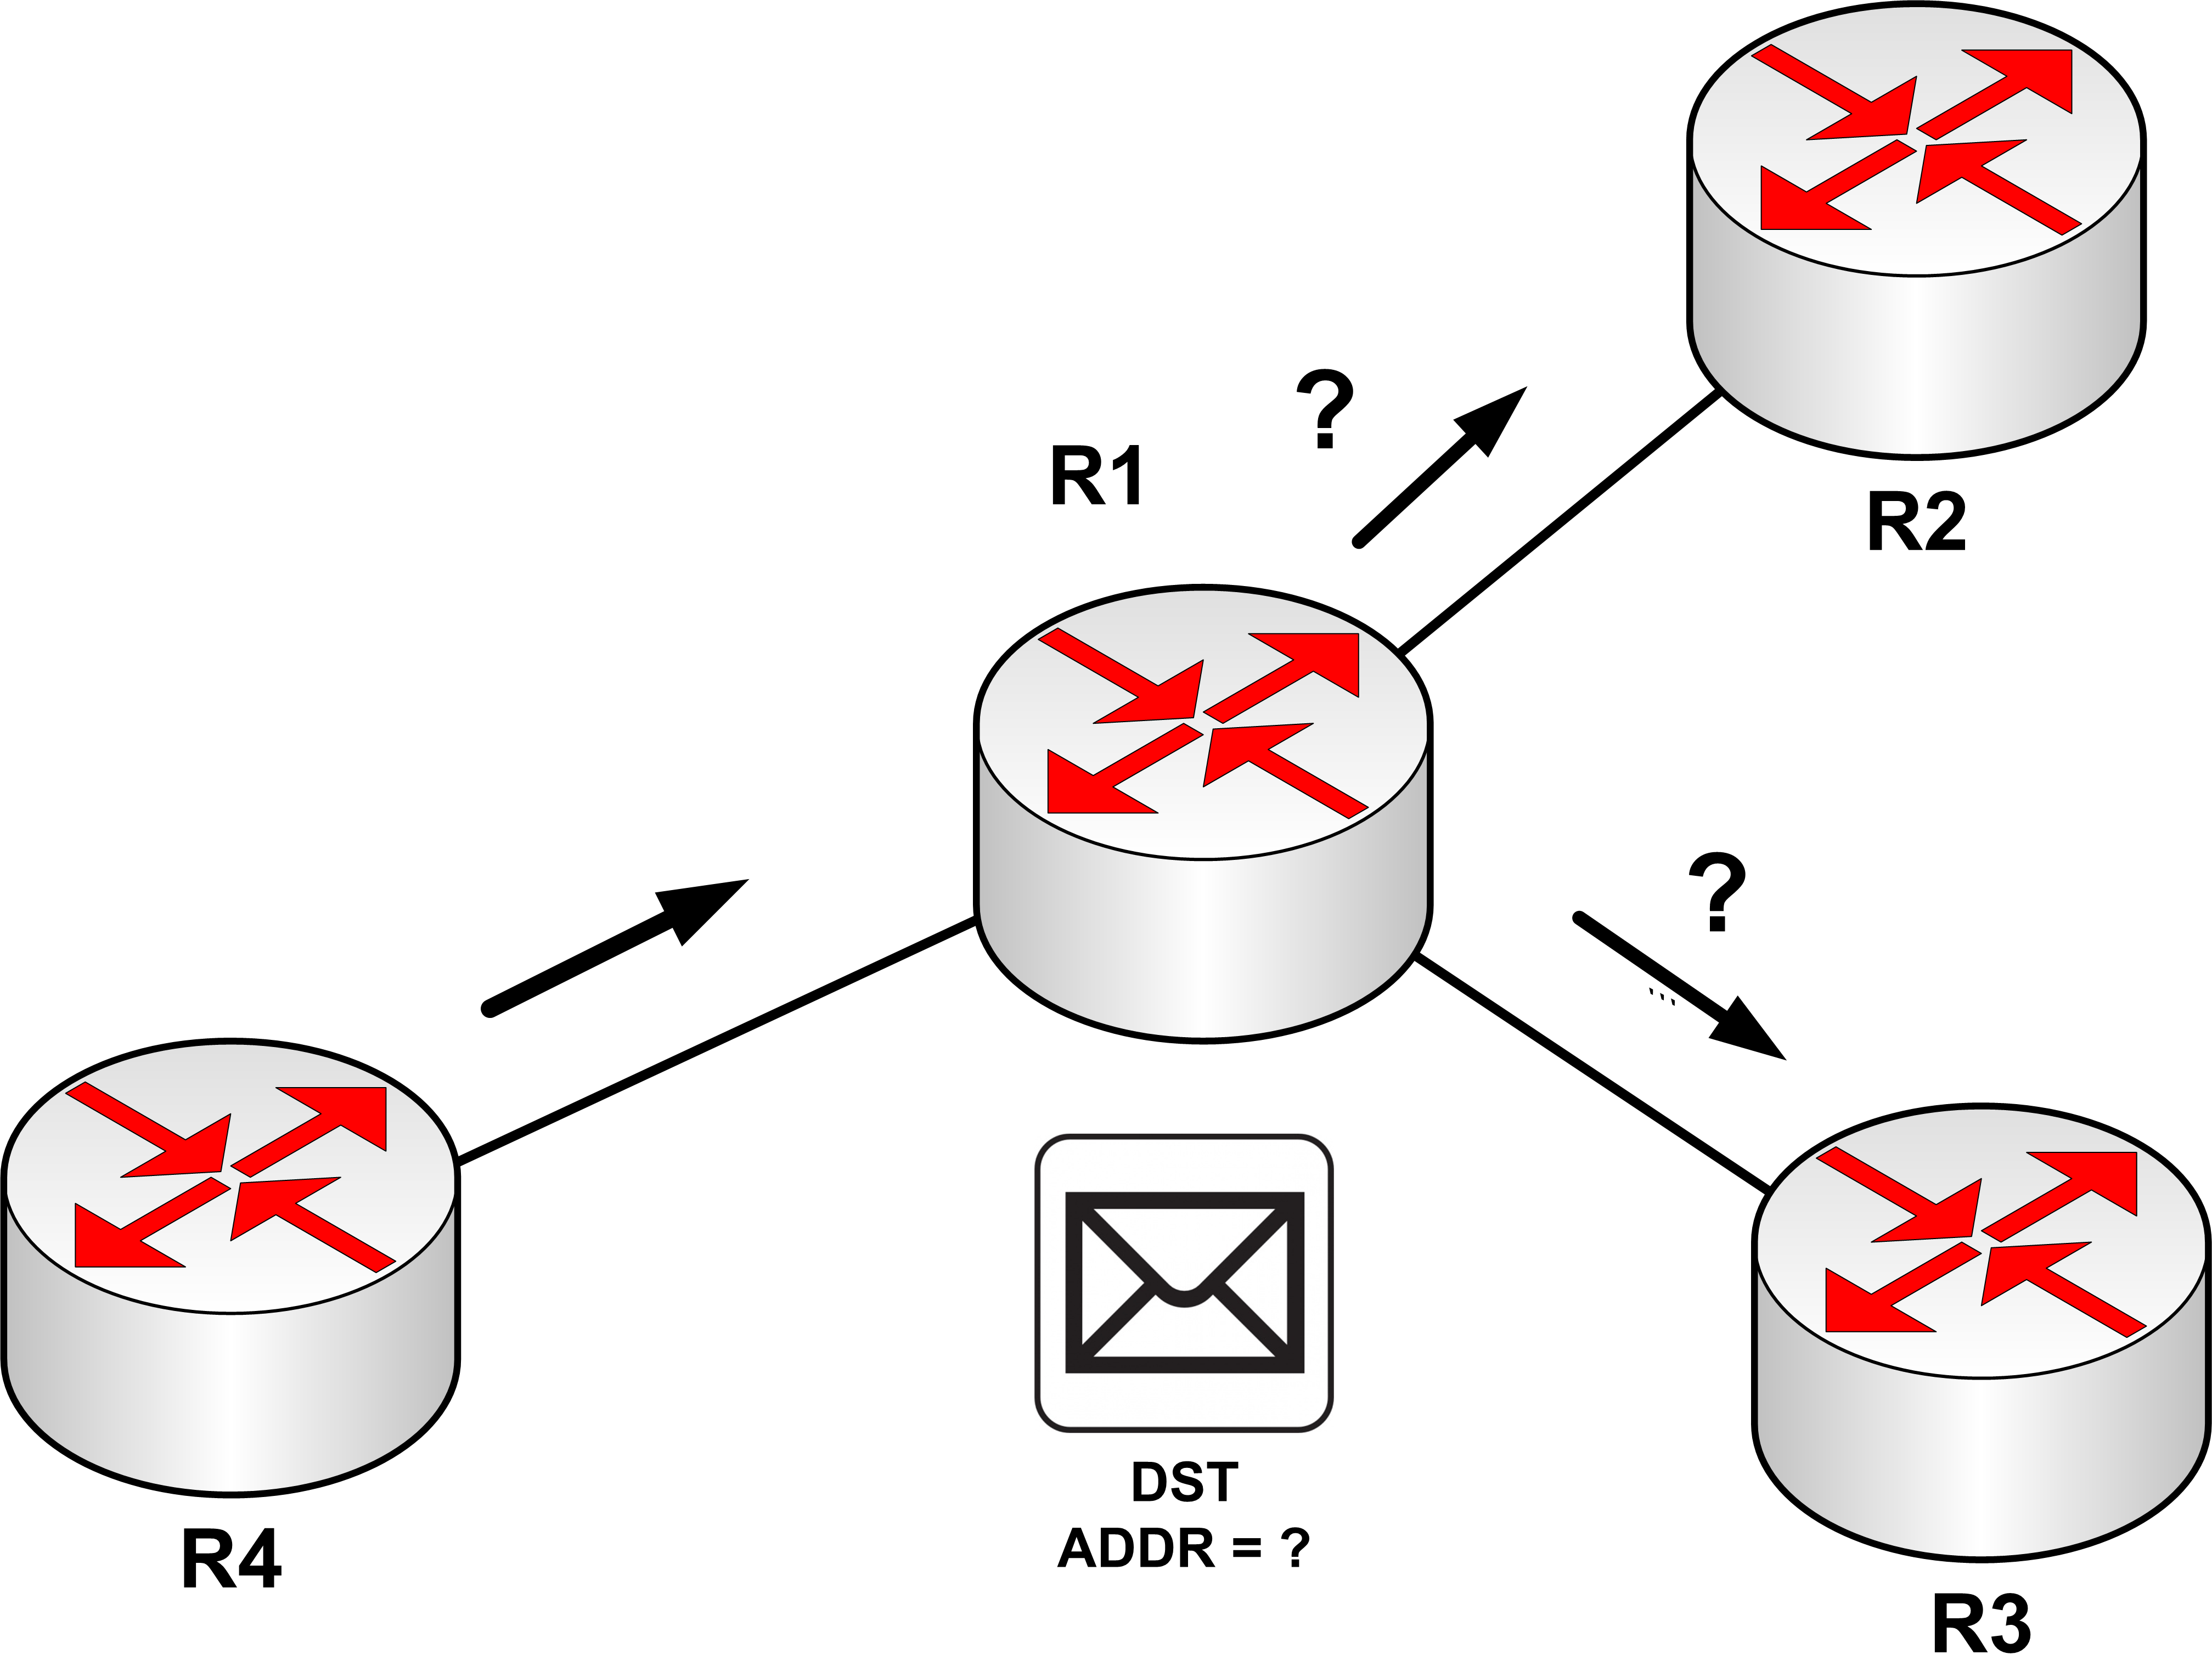
\includegraphics[width=0.50\textwidth]{images/chapter3/3-19}
 \caption {\textsl{Προώθηση Πακέτων IP}}
 \label{3-19}
\end{figure}

Πρέπει να διευκρινίσουμε ότι η διαδικασία αυτή επαναλαμβάνεται χωριστά για κάθε αυτοδύναμο πακέτο, ακόμα και αν όλα που λαμβάνονται αποτελούν τμήματα της ίδιας επικοινωνίας (σχήμα \ref{3-19}). Έτσι είναι δυνατόν IP πακέτα της ίδιας επικοινωνίας να ακολουθούν το καθένα διαφορετική διαδρομή σε άλλη χρονική στιγμή (με αποτέλεσμα βέβαια να λαμβάνονται και εκτός σειράς από τον παραλήπτη). Ένας δρομολογητής αποφασίζει μόνο για το επόμενο άλμα ενός πακέτου: \emph{η πλήρης διαδρομή δεν είναι γνωστή από την αρχή της επικοινωνίας}.

Οι πίνακες δρομολόγησης περιέχουν και πληροφορίες οι οποίες περιέχουν το βαθμό προτίμησης μια διαδρομής (του επόμενου άλματος -- next hop).

Για να επιτυγχάνεται η καλύτερη δυνατή δρομολόγηση, οι δρομολογητές ανταλλάσσουν μεταξύ τους μηνύματα και ενημερώνουν τους πίνακες δρομολόγησης τους.  Τα μηνύματα μπορεί να περιέχουν ολόκληρους πίνακες δρομολόγησης ή μέρος αυτών. Από την ανάλυση των μηνυμάτων, ένας δρομολογητής μπορεί να σχηματίσει μια ξεκάθαρη εικόνα της τοπολογίας και της τρέχουσας κατάστασης των γραμμών και των συνδέσεων του Διαδικτύου. Από τις πληροφορίες αυτές είναι σε θέση να προσδιορίζει τις βέλτιστες διαδρομές προς τους διαφορετικούς προορισμούς του Διαδικτύου.

Το πρωτόκολλο IP χρησιμοποιεί αυτοδύναμα πακέτα (datagrams) και είναι σχεδιασμένο να λειτουργεί σε όλους τους τύπους υλικού δικτύου (Ethernet, Token Ring κλπ). Πρόκειται για ένα πρωτόκολλο λογικής \emph{best effort delivery} δηλ. βέλτιστης προσπάθειας:  κάνει ότι καλύτερο μπορεί για να επιδώσει το κάθε αυτοδύναμο πακέτο, δεν παρέχει όμως εγγυήσεις π.χ. για την ταχύτητα, την καθυστέρηση, τη σειρά επίδοσης κλπ. Δεν μπορεί να αντιμετωπίσει τα παρακάτω προβλήματα:

\begin{itemize}
\item Επανάληψη αυτοδύναμου πακέτου
\item Επίδοση με καθυστέρηση ή εκτός σειράς
\item Αλλοίωση δεδομένων
\item Απώλεια αυτοδύναμου πακέτου
\end{itemize}

Για την αντιμετώπιση τέτοιων σφαλμάτων, είναι υπεύθυνα τα ανώτερα επίπεδα. Για παράδειγμα, μια επικοινωνία TCP (επίπεδο μεταφοράς) παρέχει αξιοπιστία παρά το γεγονός ότι στο επίπεδο διαδικτύου εξυπηρετείται από το πρωτόκολλο IP.

 
